\documentclass[a4paper]{book}

% 引用setting里的设置,而不直接写在这里,使代码更简洁
%% packages

\usepackage{blindtext} % needed for creating dummy text passages
%\usepackage{ngerman} % needed for German default language
\usepackage{amsmath} % needed for command eqref
\usepackage{amssymb} % needed for math fonts
\usepackage[
	colorlinks=true
	,breaklinks
	%,ngerman
	]{hyperref} % needed for creating hyperlinks in the document, the option colorlinks=true gets rid of the awful boxes, breaklinks breaks lonkg links (list of figures), and ngerman sets everything for german as default hyperlinks language
%\usepackage[hyphenbreaks]{breakurl} % ben�tigt f�r das Brechen von URLs in Literaturreferenzen, hyphenbreaks auch bei links, die �ber eine Seite gehen (mit hyphenation).
\usepackage{xcolor}
\definecolor{c1}{rgb}{0,0,1} % blue
\definecolor{c2}{rgb}{0,0.3,0.9} % light blue
\definecolor{c3}{rgb}{0.3,0,0.9} % red blue
\hypersetup{
    linkcolor={c1}, % internal links
    citecolor={c2}, % citations
    urlcolor={c3} % external links/urls
}
%\usepackage{cite} % needed for cite
\usepackage[round,authoryear]{natbib} % needed for cite and abbrvnat bibliography style
\usepackage[nottoc]{tocbibind} % needed for displaying bibliography and other in the table of contents
\usepackage{graphicx} % needed for \includegraphics 
\usepackage{longtable} % needed for long tables over pages
\usepackage{bigstrut} % needed for the command \bigstrut
\usepackage{enumerate} % needed for some options in enumerate
\usepackage{todonotes} % needed for todos
\usepackage{makeidx} % needed for creating an index
\usepackage[UTF8, heading=true]{ctex}
\makeindex
  
%% page settings

\usepackage[top=2cm, bottom=1.8cm,left=2.5cm,right=2.5cm]{geometry} % needed for page border settings
\parindent=2cm % for space of first line of new text block
\sloppy % for writing with hyphenless justification (tries to)
\hyphenation{} % 让连接词不出现在同一行
\hyphenpenalty=10000
\exhyphenpenalty=10000
\usepackage{fancyhdr} % 页眉页脚设定

%% my macros

%% Text fomats
\newcommand{\tbi}[1]{\textbf{\textit{#1}}}

%% Math fonts
\newcommand{\bbA}{\mathbb{A}}
\newcommand{\bbB}{\mathbb{B}}
\newcommand{\bbC}{\mathbb{C}}
\newcommand{\bbD}{\mathbb{D}}
\newcommand{\bbE}{\mathbb{E}}
\newcommand{\bbF}{\mathbb{F}}
\newcommand{\bbG}{\mathbb{G}}
\newcommand{\bbH}{\mathbb{H}}
\newcommand{\bbI}{\mathbb{I}}
\newcommand{\bbJ}{\mathbb{J}}
\newcommand{\bbK}{\mathbb{K}}
\newcommand{\bbL}{\mathbb{L}}
\newcommand{\bbM}{\mathbb{M}}
\newcommand{\bbN}{\mathbb{N}}
\newcommand{\bbO}{\mathbb{O}}
\newcommand{\bbP}{\mathbb{P}}
\newcommand{\bbQ}{\mathbb{Q}}
\newcommand{\bbR}{\mathbb{R}}
\newcommand{\bbS}{\mathbb{S}}
\newcommand{\bbT}{\mathbb{T}}
\newcommand{\bbU}{\mathbb{U}}
\newcommand{\bbV}{\mathbb{V}}
\newcommand{\bbW}{\mathbb{W}}
\newcommand{\bbX}{\mathbb{X}}
\newcommand{\bbY}{\mathbb{Y}}
\newcommand{\bbZ}{\mathbb{Z}}

%%%%%%%%%%%%%%%%%%%%%%%%%%%%%%%%%%%%%%%%%%%
\usepackage{hyperref}%设置超链接
\hypersetup{colorlinks, linkcolor=blue}
\usepackage{graphicx}
\usepackage{color}
\usepackage{mboxfill}
\usepackage{ctex}
\usepackage{amsmath}
\usepackage{caption}
\usepackage{amsthm}
%%%%%%%%%%%%%%%%%%%%%%%%%%%%%%%%%%%%%%%%%%%
\newcommand{\xtjc}[1]{\textbf{\textit{#1}}}
\renewcommand{\proofname}{\indent\bf 证明}%将证明两个字加粗
\makeatletter
\renewenvironment{proof}[1][\proofname]{\par
	\pushQED{\qed}%
	\normalfont \topsep6\p@\@plus6\p@\relax
	\trivlist
	\item[\hskip\labelsep
	\itshape
	#1\@addpunct{}]\ignorespaces
}{%
	\popQED\endtrivlist\@endpefalse
}
\makeatother   %去掉证明环境中证明两字后面的.
%%%%%%%%%%%%%%%%%%导言区%%%%%%%%%%%%%%%%%%%


\begin{document}

% downloaded template
\begin{titlepage}

\newcommand{\HRule}{\rule{\linewidth}{0.5mm}} % 定义横线
\center % Center everything on the page
 
%----------------------------------------------------------------------------------------
%	HEADING SECTIONS
%----------------------------------------------------------------------------------------

\textsc{\LARGE Wuhan University}\\[1.5cm] % Name of your university/college


%----------------------------------------------------------------------------------------
%	TITLE SECTION
%----------------------------------------------------------------------------------------

\HRule \\[0.4cm]
{ \huge \bfseries An Introduction to Cosmology}\\[0.4cm] % Title of your document
\HRule \\[1.5cm]
 
%----------------------------------------------------------------------------------------
%	AUTHOR SECTION
%----------------------------------------------------------------------------------------

\begin{minipage}{0.4\textwidth}
 \centering{\LARGE\textbf{猫の薛定谔} }
\end{minipage}


\vfill % Fill the rest of the page with whitespace
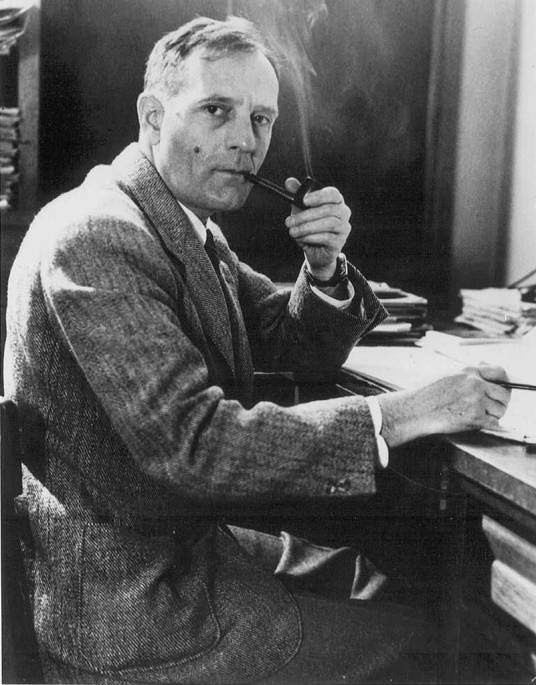
\includegraphics[width=0.5\textwidth]{figures/Hubble}\\[1cm]
\end{titlepage}



\pagestyle{plain}
\tableofcontents


%%%%%%%%%%%%%%%%%%%%%%%%%%%%%%%%%%%%%%%%%%%%%%%%%%%%%%%%%%%
%%%%%%%%%%%%%%%%%%%%%%%%%%%%%%%%%%%%%%%%%%%%%%%%%%%%%%%%%%%
%%%%%%%%%%%%%%%%%%%%%%%%%%%%%%%%%%%%%%%%%%%%%%%%%%%%%%%%%%%

\chapter{膨胀中的宇宙}
上世纪广义相对论的提出使人们理论上推衍宇宙成为可能:从广义相对论得到宇宙线性演化的解。另一方面,哈勃定律、大爆炸核合成和宇宙微波背景辐射的发现从观测上肯定了宇宙学的潜力,使得宇宙学成为一门经过实证的科学.\par 
根据观测上已经建立起来的可靠事实,我们知道我们的宇宙:\par 
\textbullet 在大于100Mpc的尺度以上是均匀且各向同性的,且在更小的尺度有高度发展的非均匀结构; \par 
\textbullet 按照哈勃定律膨胀; \par 
\textbullet 充满了温度为$T\simeq2.73K$的热微波背景辐射; \par 
\textbullet 存在重子物质,且光子数和重子数之比为$10^9$,但没有大量存在的反重子物质;\par 
\textbullet 重子物质的化学组分是:75\%的氢,25\%的氦,以及少量其他的重元素;\par 
\textbullet 重子物质的贡献只占总能量密度的百分之几;其他部分是一种暗组分,它由占25\%的暗物质\par ~(压强可忽略)和占70\%的暗能量(压强为负)组成;\par 
\textbullet 宇宙尺度为现在的千分之一时,能量密度分布上仅存在大小仅为$10^{-5}$量级的小涨落.

\section{宇宙学基本原理}
 要用物理规律系统地研究宇宙,必须先对它的整体面貌有一个基本的了解,但想要做到对宇宙有一个基本的认识是很不容易的.历史上,也有一些物理学家尝试去提出一些方程来解释这个宇宙,比如Wilhelm Herschel提出的银河系模型.但由于观测手段的限制,这些方程并没有给出一个很好的解释.\par 
 随着观测手段的进步,天文学家们发现,宇宙在足够大的尺度上是各向同性的.那么,现在我们有足够的理由相信我们的宇宙同时也是均匀的,只有一种可能无法解释这种均匀性.就是宇宙中的星系都分布在一层层的球壳之上,并且每一层的球壳上的星系分布都是各向同性的,并且我们地球就恰巧位于这些球壳的的圆心处,这样当然在各个方向的观测是各项同性的,并且非均匀的.但这种想法早在16世纪就被人提出质疑了.故我们必须相信我们的宇宙是均匀的.\par 
 
 当然你肯定会觉得,这不是扯淡吗,你说均匀性,那咱们的太阳系,不同行星间的距离,还有小行星带,就不均匀啊,你说各向同性,那咱们位于银河系的盘上,我们往银河系外看,和往银心看,肯定是不一样的啊.这就是问题的关键,这两大性质成立的前提条件就是大尺度结构,即宇宙学的基本原理应陈述为:\par 
 \centerline{\textbf{在大尺度下,任何时刻的宇宙空间都是均匀且各项同性的.}}\par 
 其中的大尺度大约是大于$10^8$光年.对于上述的问题,可以用一个不太准确的比喻来描述.当你煮了一锅汤圆,然后你用勺子搅了搅,接着给每个碗中都打了一勺汤圆.这个时候你会发现并不是每碗中的汤圆数目都是一样的,但你又看了看锅中汤圆的确是均匀分布的.而我们的宇宙就像是这个锅一样,一个个的碗就代表着一个个的星系,在小尺度下看其分布是不均匀的,但在大尺度下看,其就变得大致均匀了.在观测结果上证明了我们的猜想是可行的(图1.1).宇宙学基本原理的最有力证据就是所谓的宇宙微波背景辐射(Cosmic Microwave Background,CMB),其在在不同方向上观测到的宇宙微波背景辐射的温度分布是相同的. \par
 \begin{figure}[!h]
	\centering
	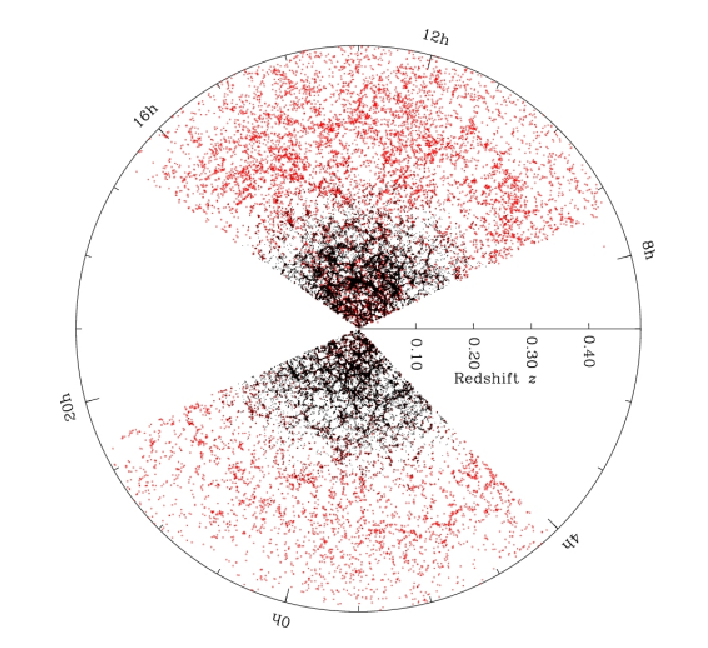
\includegraphics[width=9.36cm,height=8.4cm]{figures/宇宙的大尺度结构.eps}
     \caption{图中心为地球,可以看到在观测结果上,大尺度机构下星系基本都是均匀分布的.而随着距离增加星系的减少是由于在十分遥远的地方只有那些极为亮的星系能够被我们探测到.}
\end{figure} \par
\section{Hubble定律}
标准大爆炸模型认为宇宙由150亿年前处于一个超高温度和超高密度的均匀且各向同性的物质分布开始,经历了膨胀和冷却的过程演化至今.类似于引力场方程的推导,我们后面会从Newton的引力理论讲起,因为这样我们能抓住宇宙演化动力学的许多核心要素并帮助我们直观地解释这个过程,之后再过渡到合适的相对论处理.但在这之前,我们需要先引入一个十分重要的定律,就是所谓的Hubble定律.因为其不仅在Newton和Einstein的引力论下都成立,而且还是现代宇宙学研究的开端.\par 
\begin{figure}[!h]
	\centering
	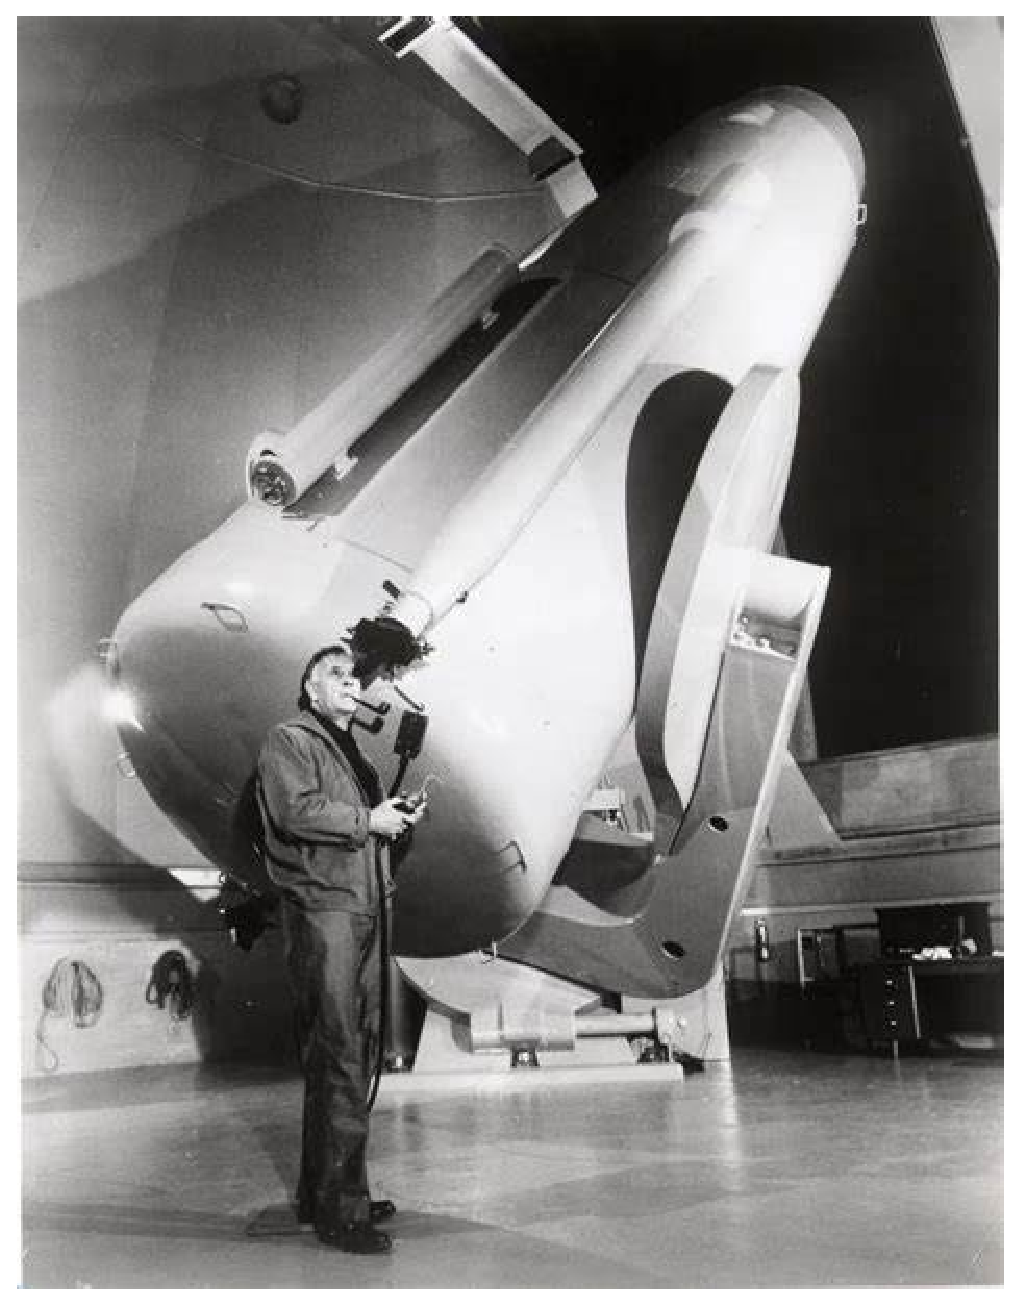
\includegraphics[width=5cm,height=7.2cm]{figures/哈勃.eps}
	\caption{星系天文学的奠基人、被誉为20世纪最伟大的天文学家Hubble,使用美国威尔逊山天文台2.5m望远镜发现了Hubble定律.不过今天的天文台中是不允许抽烟的.}
\end{figure}\par 
现在考虑宇宙内的一个区域,在大尺度结构下不同的部分间的唯一作用力仅有引力.那么考虑该区域内某一点A.现在令人困惑的是,在A点是否会发生些什么,其是向该区域内的中心加速吗?因为中心区域有一大堆物质,还是说向外加速,毕竟外围同样有很多物质.你可能下意识的认为A点就一直待在那儿.类似考虑另一点B,它的情况也与A一样,因为每个地方都和其他地方一样.故很自然的猜测就是宇宙是静态的.但这是不对的,宇宙学实际的Newton方程并不是这样的.美国天文学家Edwin Hubble发现我们的宇宙并不是静态的,而是在膨胀的.尽管你可能认为宇宙膨胀是在广义相对论下才真正被理解的,但这仅仅在历史上是正确的,但从逻辑上来讲,就像我开头所讲的那样,我们推导出动态的宇宙方程不需要依靠任何的广义相对论的知识.\par 

首先我们要做的就是引入一组坐标,如图1.3所示.那么现在我们该用什么来表示这个网格中相邻格点A、B间的\textbf{固有距离}$r_{AB}$呢?我们当然可以任意规定相邻格点间距大小,但更为明智的做法不仅仅是固定格点间的距离,而是认为这些的格点已经被选中,而星系就一直待在被选中的格点上不随时间的变化,这意味着如果宇宙真的在膨胀或者收缩,这些网格必须也要扩展或收缩.此时这些星系的坐标就被称为\textbf{共动坐标},它们间的距离就叫做\textbf{共动距离},我们设其为$\chi_{AB}$.你可能会认为如果星系像气体分子一样是做无规则运动的,那么我们建立的坐标不就不成立了吗?但当仰望夜空的时候,你会发现并不是这样,你看到的是这些星系们在非常连贯的移动,就像它们被嵌入了一个网格之中,故我们可以采取这样的坐标来完成我们的推导.现在我们进一步假设,认为固有距离$r_{AB}$与共动距离$\chi_{AB}$是成正比的
\begin{equation}\label{1.1}
	r_{AB}=a(t)\chi_{AB}
\end{equation}
可以看到,这个假设十分自然.其中$a(t)$为比例常数,我们称其为\textbf{标度因子},其可能是常数,也可能不是常数.现在对上式两边同时关于时间求导,有
\begin{equation}\label{1.2}
	\dot{r}_{AB}=v_{AB}=\dot{a}\chi_{AB}
\end{equation}
联立\hyperref[1.1]{1.1}式和\hyperref[1.2]{1.2}式,有
\begin{equation}\label{1.3}
	\frac{v_{AB}}{r_{AB}}=\frac{\dot{a}(t)}{a(t)}=H(t)
\end{equation}

\begin{figure}[!h]
	\centering
	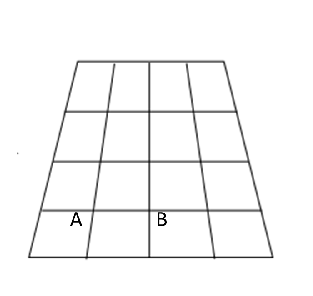
\includegraphics[width=5.36cm,height=4.4cm]{figures/坐标.eps}
	\caption{共动坐标示意图,A、B两点的坐标不随时间的变化而改变.}
\end{figure} 
可以看到A、B两点间速度与距离的比值等于$\dot{a}$与$a$的比值$H(t)$,我们称其为\textbf{Hubble常数}.尽管我们称其为“常数”,但可以看到其是与时间有关的一个量,它仅仅与坐标无关.所以其更为恰当的名字应该是“Hubble参数”或者“Hubble函数”,但按照惯例,我们还是称其为Hubble常数.上述A、B两点位置的选取是随意的,我们可以把该结论推广到宇宙中任意两个星系
\begin{equation}\label{1.4}
	\xtjc{v}=H(t)\xtjc{r}
\end{equation}
这就是著名的 \textbf{Hubble 定律},不难发现,这个定律与宇宙学基本原理相处的十分融洽.事实上,它也是唯一与均匀且各项同性相容的膨胀率.\par 
\begin{figure}[!h]
	\centering
	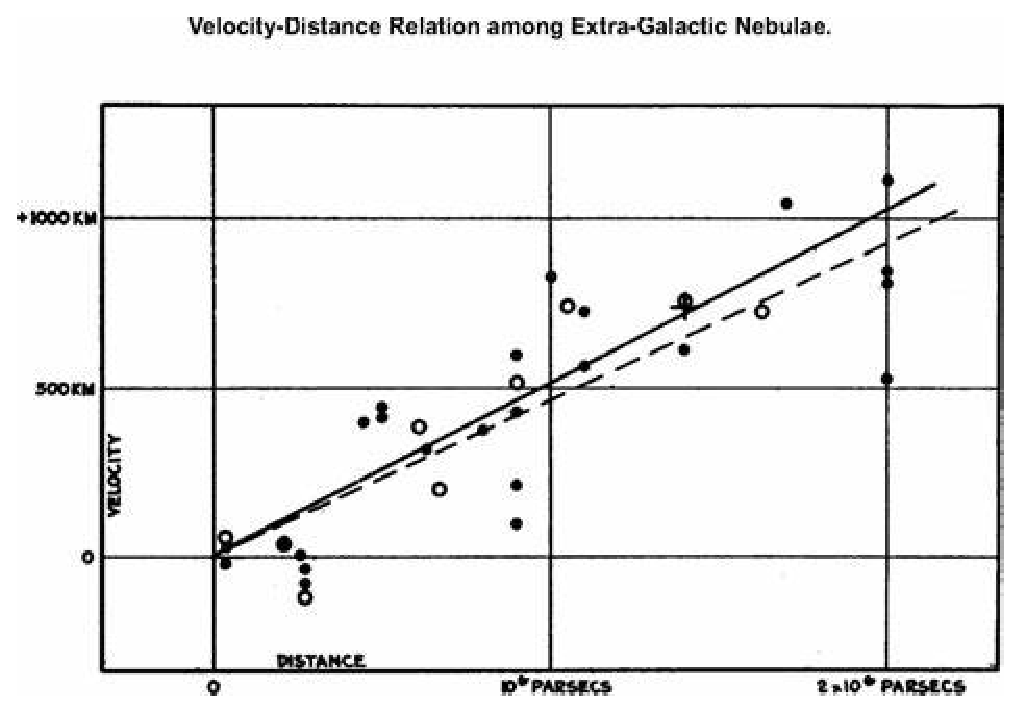
\includegraphics[width=10cm,height=7cm]{figures/观测.eps}
	\caption{Hubble当年给出的速度-距离关系图.图中实点代表星系,实线是对观测星系的拟合线;圆圈代表这些星系按方向和距离的分组,虚线是对这些组的拟合线.}
\end{figure}
在这种描述中,我们假设宇宙是完美地均匀且各向同性的.但在真实的宇宙中,在物质发生聚合的地方,附近物体的运动并不是由引力所主导的.这会产生位力轨道运动之类的,而不是Hubble膨胀.类似地,物体本身是靠其他更强的力聚合在一起抵抗Hubble膨胀.这类物体相对于观测者的速度被称为\textbf{本动速度}.因此,Hubble定律仅在均匀性成立下的尺度上是有效的.\par 
Hubble常数在目前时刻的值$H_0$可以通过测量那些本动速度远小于共动速度的遥远天体的退行速度与距离之比来得到.退行速度会产生多普勒红移,因此其可以测量的很准确.比较困难的是天体距离的测量,由于测量天体的距离几乎都在银河系之外,故我们不能采用常见的三角视差法(见附录B)来测量这些天体的距离.现比较常用的方法是基于所谓的“\textbf{标准烛光}”.如果一组天体的光度差不多相同,就可以当做标准烛光.它们通常具有一些特性,使我们在十分遥远的距离能认出它们.而我们只要把观测到的标准烛光星体与已经校准的标准烛光作比较就可以测量出它们的距离.较为常见的标准烛光为\textbf{造父变星}和\textbf{IA型超新星}.造父变星是由于大质量的恒星演化到晚期时发生不稳定的脉冲现象形成脉动变星,其光度会发生周期性的变化,让天文学家在遥远的地方能认出来.IA型超新星的光谱型比较特殊,其有强硅线而没有氢线.由于系统误差的不确定性的影响,目前哈勃常数测量的精度值不高,大约在$65\sim80km\cdot s^{-1}\cdot Mpc^{-1}$.
\begin{figure}[!h]
	\centering
	\includegraphics[width=15cm,height=4cm]{figures/标准烛光.eps}
	\caption{左图为造父变星光度随时间的变化,其中横坐标为时间,纵坐标为光度;右图为IA型超新星光谱.}
\end{figure}\par 
可以看到,Hubble定律的起源为运动学,而且它的形式完全是均匀且各项同性的性质所要求的,所以它对Newton理论和广义相对论都成立.实际上,按照\hyperref[1.1]{1.1}式所重写的Hubble定律可以直接运用于Einstein的引力理论.这一点可能会令人困惑,因为按照Hubble定律,两个距离超过$1/H$的物体之间的相对速度可以超过光速.这不是违背狭义相对论吗?这是因为在广义相对论里距离超过$1/H$(时空的曲率尺度)的物体之间的相对速度没有相对论不变性的意义.之后我们会在Milne宇宙的那一节进一步讨论该问题.
\section{Newton宇宙学中的动力学}
我们在进行Newton宇宙学中的一系列推导前需要引入一个重要的定理,就是所谓的“Birkhoff定理”与“壳层定理”,前者指对于均匀物质分布的球体,其表面粒子受到的引力与所有物质都集中在其中心上的引力相同;后者指位于物质球壳内的物体不会受到来自球壳的静引力。这两个定理合在一起构成了经典力学中的Newton定理.而这个定理能够直观地推出一个重要的结论,即
\centerline{\textbf{位于一个均匀物质分布球体表面的粒子,其受到来自球面外物质的总作用为0.}}\par 
下面我们考虑的都是一个无限大且正在膨胀的均匀且各向同性的宇宙,其中充满了非相对论性的物质,即压强相对于其能量密度可以忽略的物质类型.我们先任选一点作为坐标原点,并考虑它周围的一个半径为$R(t)=a(t)\chi_{AB}$的膨胀的球面.假设引力\textbf{很弱},且半径\textbf{足够小},使得球面粒子相对于原点的速度远小于光速,那么其膨胀就可以用Newton引力来处理.在推导前必须一提的是,下列推导并不完全严格,但这并不是我们关心的问题.因为我们所要了解的就是牛顿宇宙学与相对论宇宙学能如此相像的基础就是宇宙学基本原理.\par 
\subsection{连续性方程}
球内的总质量M是守恒的.故其物质密度为
\begin{equation}
	\rho(t)=\frac{M}{(4\pi/3)R^3(t)}=\rho_{0}\Big[\frac{a_0}{a(t)}\Big]^3
\end{equation}
其中$\rho_{0}$为标度因子等于$a_0$时刻的物质密度.对上式两边做时间导数,有
\begin{equation}\label{1.6}
	\dot{\rho(t)}=-3\rho_{0}\Big[\frac{a_0}{a(t)}\Big]^3\frac{\dot{a}}{a}=-3H\rho(t)
\end{equation}
实际上这个就是连续性方程的表达形式,只要我们在连续性方程
\begin{equation}
	\frac{\partial\rho}{\partial t}+\nabla\cdot(\rho\xtjc{v})=0
\end{equation}
中令$\rho(\xtjc{r},t)=\rho(t)$与$\xtjc{v}=H\xtjc{r}$就可以得到.从连续性方程出发,并假设均匀的初始条件,可以直接看出在随时间演化过程中保持均匀性的唯一速度分布就是Hubble定律.\hyperref[1.6]{1.6}式是我们得到的第一个动力学方程.\par 
\subsection{加速方程}
物质之间存在相互吸引的万用引力作用,这使得宇宙的膨胀减速.为了推导出标度因子的运动方程,考虑一个位于球表面的质量为$m$的粒子,它到原点的距离为$R(t)$.由Newton第二定律有
\begin{equation}
	m\ddot{R}=-G\frac{mM}{R^2}=-\frac{4\pi}{3}Gm\frac{M}{(4\pi/3)R^3}R
\end{equation}
利用\hyperref[1.5]{1.5}式中定义的物质密度,并代入$R(t)=a(t)\chi$,有
\begin{equation}
	\ddot{a}=-\frac{4\pi G}{3}\rho a
\end{equation}
最后的结果中的粒子质量和球面共动坐标都消掉了.这是我们得到的第二个动力学方程.
\subsection{牛顿解}
宇宙中物质的运动必然是在力的作用下,而目前所考虑的力也只有引力,也就是说,目前天体的退行运动是由于宇宙中物质的引力作用所引起的.忽略掉压力的影响,引力可以用Poisson方程来表示
\begin{equation}\label{1.10}
	\nabla \cdot \xtjc{F}=-4\pi G\rho
\end{equation}
考虑宇宙中单位质量物质的加速运动,可写为
\begin{equation}
	\xtjc{F}=\frac{d\xtjc{v}}{dt}
\end{equation}
对\hyperref[1.4]{1.4}式两边微分,有
\begin{equation}
	\frac{d\xtjc{v}}{dt}=\xtjc{r}\Big[\frac{dH}{dt}+H^2\Big]
\end{equation}
对上式两边同时作用一个$\nabla$算符,并将\hyperref[1.4]{1.4}式代入,则有
\begin{equation}
	\Big[\frac{dH}{dt}+H^2\Big]\nabla\cdot\xtjc{r}=-4\pi G\rho
\end{equation}
又$\nabla\cdot\xtjc{r}=3$,故上式变为
\begin{equation}
	\frac{dH}{dt}+H^2=-\frac{4}{3}\pi G\rho
\end{equation}
我们感兴趣的事$R(t)$,将\hyperref[1.4]{1.4}式代入上式,并考虑到$v=\frac{dR}{dt}$有
\begin{equation}
	\frac{1}{R}\frac{d^2R}{dt^2}+\frac{4}{3}\pi G\rho=0
\end{equation}
其表明,只要宇宙不是真空的,即$\rho \ne 0$,宇宙便不可能处于静止状态,加速度是必然的.将上式两边乘以$2R\frac{dR}{dt}$,有
\begin{equation}\label{1.16}
2\frac{dR}{dt}\frac{d^2R}{dt^2}+\frac{8}{3}\pi G\rho\frac{dR}{dt}R=0
\end{equation}
在宇宙学基本原理的条件下,假定宇宙中的物质总质量不会变,有
\begin{equation}\label{1.17}
	\rho(t)R(t)^3=\rho(t_0) R(t_0)^3\equiv\rho_0
\end{equation}
联立\hyperref[1.6]{1.6}式和\hyperref[1.7]{1.7}式,有
\begin{equation}
	2\frac{dR}{dt}\frac{d^2R}{dt^2}+\frac{8}{3}\pi G\rho_0\frac{1}{R^2}\frac{dR}{dt}R=0
\end{equation}
而上式刚好是对t的一个完整积分
\begin{equation}
	\frac{d}{dt}\Big[\Big(\frac{dR}{dt}\Big)^2-\frac{8\pi G}{3}\rho_0 \frac{1}{R}\Big]=0
\end{equation}
将$\rho_0$以$\rho R^3$代替,可以得到
\begin{equation}
\Big(\frac{dR}{dt}\Big)^2-\frac{8\pi G}{3}\rho R^2=-k
\end{equation}
其中$k$为积分常数.考虑\hyperref[1.1]{1.1}式与\hyperref[1.4]{1.4}式,有
\begin{equation}
	H^2+\frac{k}{a^2}=\frac{8\pi G}{3}
\end{equation}
这就是我们得到的最后一个方程.\par 
本节我们并没有进行过多的讲解,仅仅是推导出了一些基本的公式.更多详细的讲解我们会放到下一节来讲述.我们将会就看到,用牛顿力学得到的结果,与广义相对论的结果基本相同,这归功于宇宙学原理.宇宙学原理告诉我们,宇宙各个局部的运动状态都是一样的,因此我们可以在一个足够小的局部范围内来研究宇宙膨胀运动.在小范围内,星体的相对运动速度小于光速$c$,所以可以应用牛顿理论.而对于大尺度的问题,如高红移天体、距离、光度等,牛顿力学就不适用了.
\section{从Newton宇宙到相对论宇宙}
广义相对论可以推出数学上自洽的宇宙理论,但Newton理论不行.并且广义相对论相比于Newton描述还能带来一系列重要的变化.首先,Einstein的理论指出几何是动力学的,且为宇宙的物质成分所决定.其次,广义相对论能描述以相对论性的速度运动并且具有任意压强的物质.我们知道在大爆炸之后的10万年内,宇宙是由压强等于其能量密度的三分之一的辐射主导的.此外,有证据表面在今天大多数的能量密度具有负压强.为了理解这些宇宙历史中重要的时间段,我们只能超出Newton引力的范畴而转向完全相对论性的理论.
\subsection{均匀及各向同性空间的几何}
我们先考虑哪种三维空间可以用来描述一个均匀且各向同性的宇宙.我们的宇宙的演化可以表示为一系列按时间顺序排列的三维类空超曲面,其中每张超曲面都是均匀且各向同性的.这些超曲面可自然地选为等时面.\par 
均匀且各向同性的空间具有最大可能的对称群.在三维里,有三种独立的平移和三种转动.这些对称性强烈地限制了这类空间的可允许的几何,只存在三种类型的带有简单拓扑的均匀且各向同性的空间:(a)平坦空间,(b)常数正曲率的三维球,(c)常数负曲率的双曲空间.\par 
为了便于理解,我们考虑预与之类似的二维的均匀且各向同性的曲面,将其推广到三维是直截了当的.两种均匀且各向同性的曲面是平面和二维球面.它们都可以嵌入到带有通常Cartesian坐标$x$,$y$,$z$的三维Euclid空间之中,描述二维球面的嵌入的方程为:
\begin{equation}
	x^2+y^2+z^2=a^2
\end{equation}
其中$a$为球的半径.对上式做微分,有
\begin{equation}
	dz=-\frac{xdx+ydy}{z}=\pm \frac{xdx+ydy}{\sqrt{a^2-x^2-y^2}}
\end{equation}
将上式代入Euclid度规
\begin{equation}
	dl^2=dx^2+dy^2+dz^2
\end{equation}
中,我们得到
\begin{equation}
	dl^2=dx^2+dy^2+\frac{(xdx+ydy)^2}{a^2-x^2-y^2}
\end{equation}
以这种方式,位于二维球面上的两点之间的距离就完全用两个约束在$x^2+y^2\leq a^2$上的独立坐标$x$和$y$表示出来了.然而这两个坐标是退化的,也就是说,任意一组给定$(x,y)$对应预球面上南半球和北半球的两个点.相比于$x$和$y$,更方便的是引入角坐标$r'$和$\varphi $,按照下式来定义:
\begin{equation}
	x=r'cos\varphi ,~~y=r'sin\varphi
\end{equation}
对$x^2+y^2=r'^2$作微分,我们得到
\begin{equation}
	xdx+ydy=r'dr'
\end{equation}
由此可以得到
\begin{equation}\label{1.28}
	dl^2=\frac{dr'^2}{1-(r'/a)^2}+r'^2d\varphi^2
\end{equation}
引入重标度的坐标$r=r'/\sqrt{\lvert a^2 \rvert}$,我们可以将度规\hyperref[1.28]{1.28}式改写为如下形式
\begin{equation}
	dl^2=a^2\Big(\frac{dr^2}{1-kr^2}+r^2d\varphi^2\Big)
\end{equation}
其中$k$称为空间曲率.$k=+1$对应于球面$(a^2>0),$$k=0$对应于平面(二维平坦空间),$k=-1$对应于赝球面$(a^2<0)$.$a^2<0$的空间称为Lobachevski空间.与二维平面或球面不同的是,Lobachevski空间没办法嵌入到三维Euclid空间中,因为其半径是个虚数.当然这并不意味着这类空间不能存在.如曲面$x^2+y^2-z^2=-a^2$(图1.6),采用类似的方法将其嵌入到度规为$dl^2=dx^2+dy^2-dz^2$的空间中就能给出Lobachevski空间.
\begin{figure}[!h]
	\centering
	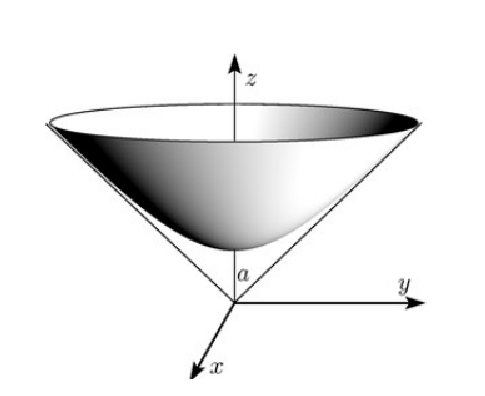
\includegraphics[width=6cm,height=6cm]{figures/双曲面.eps}
	\caption{}
\end{figure}\par 
同样的,采用相同的方法,我们可以将三维球面$x^2+y^2+z^2+t^2=a^2$或三维赝球面$x^2+y^2+z^2-t^2=a^2$嵌入到四维Euclid空间或Lorentz空间中得到三维常曲率空间的度规为
\begin{equation}\label{1.30}
	dl^2=a^2\Big(\frac{dr^2}{1-kr^2}+r^2(d\theta^2+sin^2\theta d\varphi^2)\Big)
\end{equation}
其中$a^2$为正,$k=0,\pm1$.通过
\begin{equation}
	r=\frac{\tilde{r}}{1+k\tilde{r}^2/4}
\end{equation}
引入重标度的半径坐标$\tilde{r}$,可以将度规重新写为均匀且各向同性的形式:
\begin{equation}
	dl^2=a^2\frac{d\tilde{x}^2+d\tilde{y}^2+d\tilde{z}^2}{(1+k\tilde{r}^2/4)}
\end{equation}
其中
\begin{equation}
	\tilde{x}=\tilde{r}sin\theta cos\varphi,~~	\tilde{y}=\tilde{r}sin\theta sin\varphi,~~\tilde{z}=\tilde{r}cos\theta
\end{equation}\par 
在许多情况下,与其使用半径坐标$r$,更方便的是使用以下定义的新坐标$\chi$:
\begin{equation}
	d\chi^2=\frac{dr^2}{1-kr^2}
\end{equation}
不难发现
\begin{equation}
	\chi=\left\{\begin{array}{l l}{{\mathrm{arcsinh}\,r,}}&{{k=-1}}\\ {{r,}}&{{k=0}}\\ {{\mathrm{arcsin}\,r}}&{{k=+1}}\end{array}\right.
\end{equation}
坐标$\chi$在平直和双曲空间下可取0到$+\infty$之间的值,而在正曲率的情况下的取值范围是$0\leq \chi \leq \pi$.后面这种情况下任意一个给定的$r$都对应于两个不同的$\chi$.因此引入坐标$\chi$就消除了之前谈到过的坐标退化.用$\chi$作坐标,度规\hyperref[1.30]{1.30}式可写为
\begin{equation}\label{1.36}
	d l^{2}=a^{2}(d\chi^{2}+\Phi^{2}(\chi)d\Omega^{2})\equiv a^{2}\left[d\chi^{2}+\left(\begin{array}{c}{{\sinh^{2}\chi}}\\ {{\chi^{2}}}\\ {{\sin^{2}\chi}}\end{array}\right)d\Omega^{2}\right]\begin{array}
		{c}{k=-1}\\{k=0}\\{k=+1}
	\end{array}
\end{equation}
其中
\begin{equation}
	d\Omega^2=d\theta^2+sin^2\theta d\varphi^2
\end{equation}\par 
我们现在进一步考察常曲率空间的性质.\par
\textbf{三维球面~$(k=+1)$} ~从\hyperref[1.36]{1.36}式可以看出,在一个正曲率的三维空间中,半径为$\chi$的二维球面的距离元为
\begin{equation}
	dl^2=a^2sin^2\chi (d\theta^2+sin^2\theta d\varphi^2)
\end{equation}
这个表达式和三维平直空间中半径为$R=asin\chi$的球面的结果相同,因此我们可以求出其表面积
\begin{equation}
	S=4\pi R^2=4\pi a^2sin^2\chi
\end{equation}
随着半径的增长其表面积先增长,在$\chi=\pi/2$时达到最大值,然后开始逐渐减小,并在$\chi=\pi$时减为0(图1.7).\par 
\begin{figure}[!h]
	\centering
	\includegraphics[width=10cm,height=6.5cm]{figures/表面积.eps}
	\caption{不同曲率的三维球面的表面积随半径的变化.}
\end{figure}\par 
为了理解如此诡异的表面积的演化规律,我们可以来类比低维情况.我们考虑一个二维球面.从对应于$\theta=0$的北极开始,随着我们向南移动,其对应圆环的周长逐渐增大,在$\theta=\pi/2$的时候到达最大值.之后变开始减小,在到达南极时减为0.\par 
实际上,因为无限小的壳的物理宽度是$dl=ad\chi$,故体积元的大小为
\begin{equation}
	dV=Sdl=4\pi^3sin^2\chi d\chi
\end{equation}
因此,$\chi=\chi_0$的球面的总体积是
\begin{equation}
	V(\chi_0)=4\pi a^3\int^{\chi_0}_{0}sin^2\chi d\chi=2\pi a^3\Big(\chi_0-\frac{1}{2}sin2\chi_0 \Big)
\end{equation}
在$\chi_0\ll 1$时,有
\begin{equation}
V(\chi_0)=\frac{4\pi(a\chi_0)^3}{3}+\cdots
\end{equation}
还是考虑二维球面的那个例子,当$\theta$从0变到$\pi$时,它扫过了整个球面.类似地,当$\chi$从0变到$\pi$时,它也扫过整个三维球面空间,故其总体积为$\chi=\pi$时的大小
\begin{equation}
	V_{total}=2\pi^2 a^3
\end{equation}
三维球面另一个有趣的性质是利用测地线构造出的三角形内角和小于180°.\par
\textbf{三维赝球面~$(k=-1)$}~三维常负曲率空间中半径为$\chi$的二维球面的度规是
\begin{equation}
	dl^2=a^2sinh^2\chi (d\theta^2+sin^2\theta d\varphi^2)
\end{equation}
球面的面积为
\begin{equation}
	S=4\pi a^2sinh^2\chi
\end{equation}
在$\chi\gg1$的情况下指数式增长.其体积为
\begin{equation}
	V=4\pi a^3sinh2\chi_0
\end{equation}
因为坐标$\chi$可以从0变到$\infty$,所以双曲空间的总体积是无限的.其三角形内角和小于180°.
\subsection{Einstein方程和宇宙演化}



%%%%%%%%%%%%%%%%%%%%%%%%%%%%%%%%%%%%%%%%%%%%%%%%%%%%%%%%%%%
%%%%%%%%%%%%%%%%%%%%%%%%%%%%%%%%%%%%%%%%%%%%%%%%%%%%%%%%%%%
%%%%%%%%%%%%%%%%%%%%%%%%%%%%%%%%%%%%%%%%%%%%%%%%%%%%%%%%%%%

\begin{appendix}
	
\chapter{广义相对论简介}
\label{app_ex1}
\section{等效原理}
由于惯性质量与引力质量相等,这意味着自由落体的观测者无法分辨自己是否受到引力场的影响.换句话说,引力场和惯性力场的动力学效应局部不可分辨.但这只是等效原理的弱形式,其仅建立在惯性质量与引力质量相等的物理基础上,故Einstein将这个概念推广,认为任何物理规律都是局部不可分辨的.其可严格表述为:\par
\centerline{\textbf{引力场中的任一时空点,当采用局部惯性系时,除引力外的一切物理学规律应是Lorentz协变的.}}\par 
这个原理就让我们能够在时空中任意一点的伴随惯性系下写出一组协变的方程,就可以推广至引力场的情况中.尽管这种推广通常会产生多种结果,但如果我们把自己限制在一个时空区域内,该区域内距离与时间尺度变化与引力场或其他场相比十分小,这些差异就可以忽略不计.
\section{广义相对性原理与广义协变原理}
在狭义相对论中我们曾学过:\textbf{物理定律在任何惯性系下形式不变},Einstein提出将这个概念修改为广义相对性原理,即\textbf{一切参考系都应是平权的,物理定律在任何参考系下形式不变.}\par
但数学上这个原理并不容易实现.于是将其改为数学上更容易实现的广义协变原理:\textbf{在任何坐标下的变换,物理定律都是协变的。}这边值得思考的一个问题是:什么是物理量?什么是物理定律?
\centerline{\xtjc{Answer}:\textbf{物理量是由与坐标无关的几何量描述的,物理定律是这些几何量之间的几何关系.}}\par 
有了这个,我们就可以很好的实现物理公式在不同坐标系下的变换了,后面我们会看到,只需要将局域惯性系中的方程的闵氏度规与普通导数替换为引力场下的度规与协变导数就可以得到引力场下的方程了.
\section{度规}
对于一个任意引力场下的时空,我们需要定义时空中两点的间距,此时需要引入一个非退化的、对称的二阶协变的张量场,记作$g_{\mu\nu}$,并以此定义时空间距为:
\begin{equation}\label{A.1}
	ds^{2}\equiv -d\tau^{2}=g_{\mu\nu}dx^{\mu}dx^{\nu}
\end{equation}
\par 
其中$d\tau$为固有时,即观测者所携带的时钟所走的时间.特别的,对于光线,有:
\begin{equation}
	g_{\mu\nu}dx^{\mu}dx^{\nu}=0
\end{equation}\par 
当$x^\mu$坐标系变换到$\tilde{x}^\mu$坐标系下时,度规张量有如下变换关系:
\begin{equation}
 \tilde{g}_{\mu\nu}=\frac{\partial x^{\rho}}{\partial\tilde{x}^{\mu}}\frac{\partial x^{\sigma}}{\partial \tilde{x}^{\nu}} g_{\rho\sigma} 
\end{equation}\par 
由此可以注意到\hyperref[A.1]{A.1}式是广义协变的,因为不同坐标系下有如下变换:
\begin{equation}
	d\tilde{x}^{\rho}=\frac{\partial \tilde{x}^{\rho}}{\partial x^{\mu}} dx^{\mu}
\end{equation}\par 
故
\begin{align}
	\tilde{g}_{\rho\sigma}d\tilde{x}^{\rho}d\tilde{x}^{\sigma}=
	{}& \frac{\partial x^{\mu}}{\partial \tilde{x}^{\rho}}\frac{\partial x^{\nu}}{\partial \tilde{x}^{\sigma}}g_{\mu\nu}\frac{\partial \tilde{x}^{\rho}}{\partial x^{\mu}}dx^{\mu}\frac{\partial \tilde{x}^{\sigma}}{\partial x^{\nu}}dx^{\nu} \notag \\
	={}&  g_{\mu\nu}dx^{\mu}dx^{\nu}
\end{align}\par 
可以看到,其在不同坐标系下有相同的形式.
\section{张量、矢量与标量}
满足类似于
\begin{equation}
	 \tilde{g}_{\mu\nu}=\frac{\partial x^{\rho}}{\partial\tilde{x}^{\mu}}\frac{\partial x^{\sigma}}{\partial \tilde{x}^{\nu}} g_{\rho\sigma}  \notag
\end{equation}\par 
和
\begin{equation}
	d\tilde{x}^{\rho}=\frac{\partial \tilde{x}^{\rho}}{\partial x^{\mu}} dx^{\mu} \notag
\end{equation}\par
的我们分别称其为协变张量和逆变矢量.通常逆变与协变分别由上指标和下指标表示.对于逆变其坐标变换中存在$\frac{\partial \tilde{x}}{\partial x}$;对于协变,其坐标变换中存在$\frac{\partial {x}}{\partial \tilde{x}}$。当然,混合的指标也是存在的,最为典型的就是Kronecker张量,定义为:
\begin{equation}
	\delta^{\mu}_{\nu}=\left\{\begin{array}{l l}{{1}}&{{ \mu=\nu}}\\ {{0}}&{{ \mu\not=\nu}}\end{array}\right.
\end{equation}\par
而且这个张量有个特别的地方就是其在任何坐标系下都有相同的分量:
\begin{equation}
	\tilde{\delta}^{\rho}_{\sigma}=\frac{\partial \tilde{x}^{\rho}}{\partial x^{\mu}}\frac{\partial x^{\nu}}{\partial \tilde{x}^{\sigma}}	\delta^{\mu}_{\nu}=\frac{\partial \tilde{x}^\rho}{\partial \tilde{x}^\sigma}=\left\{\begin{array}{l l}{{1}}&{{ \rho=\sigma}}\\ {{0}}&{{ \rho\not=\sigma}}\end{array}\right. \notag
\end{equation}\par 
借助这个张量,我们可以得到逆变的度规张量,其定义为$g_{\mu \nu}$的逆:
\begin{equation}
	g^{\mu \rho}g_{\rho \nu}=\delta^{\mu}_{\nu}
\end{equation}\par 
在不同坐标下,其变换自然满足:
\begin{equation}
	\tilde{g}^{\mu\nu}=\frac{\partial \tilde{x}^{\mu}}{\partial x^{\rho}}\frac{\partial \tilde{x}^{\nu}}{\partial x^{\sigma}} g^{\rho\sigma}  
\end{equation}\par
最后我们来看看标量.标量是一种在坐标变换下不变的参数,记作$S(x)$,其有
\begin{equation}
	\tilde{S}(\tilde{x})=S(x)
\end{equation}\par 
标量关于坐标的导数构成了一个协变矢量(其实就是所谓的Nabla算符$\nabla$):
\begin{equation}
	\tilde{v}_{\rho}\equiv \frac{\partial \tilde{S}}{\partial x^{\rho}}=\frac{\partial S}{\partial x^{\mu}}\frac{\partial x^\mu}{\partial \tilde{x}^\rho}=\frac{\partial x^\mu}{\partial \tilde{x}^\rho} v_{\mu} \notag
\end{equation}\par 
我们可以通过直积的方法构造新的张量:
\begin{equation}
	C^{\mu}_{\nu \rho \sigma}\equiv A^{\mu}_{\nu}B_{\rho \sigma}
\end{equation} \par 
或者我们也可以通过上下指标抵消的方式来得到新的张量,这通常发生在与度规张量或其逆的内积之间:
\begin{equation}
	A^{\nu}_{\rho}=g_{\mu \rho}A^{\mu \nu}
\end{equation}
\begin{equation}
	B^{\nu\rho}=g^{\mu \rho}A^{\nu}_{\mu}
\end{equation}\par 
注意,升高又降低同一指标得到的是原来的那个张量:
\begin{equation}
	g^{\sigma \rho}(g_{\mu \rho}A^{\mu \nu})=A^{\sigma \nu}
\end{equation} \par 
两个张量间可以作加法、减法和乘法运算.由于决定张量变换行为的矩阵是虽不同点的运算而不同的,所以必须在同一点上的两个张量间进行运算,才能使运算后的量保持张量的性质.
\newpage
\section{仿射联络}
对于坐标$x^{\mu}$的关于某个标量$u$的一阶导$\frac{dx^{\mu}}{du}$显然是一个矢量:
\begin{equation}
	\frac{d\tilde{x}^{\rho}}{du}=\frac{\partial \tilde{x}^{\rho}}{\partial x^{\mu}}\frac{dx^{\mu}}{du}
\end{equation}\par 
但其二阶导数却不是:
\begin{equation}
	\frac{d^2 \tilde{x}^{\rho}}{du^2}=\frac{d}{du}(\frac{d\tilde{x}^{\rho}}{du分母})=\frac{d}{du}(\frac{\partial \tilde{x}^{\rho}}{\partial x^{\mu}}\frac{dx^{\mu}}{du})=\frac{\partial \tilde{x}^{\rho}}{\partial x^{\mu}}\frac{d^2 x^{\mu}}{du^2}+\frac{\partial^2 \tilde{x}^\rho}{\partial x^{\mu} \partial x^{\nu}}\frac{dx^{\mu}}{du}\frac{dx^{\nu}}{du}
\end{equation}\par
这意味着我们所熟知的描述自由粒子运动的方程$\frac{d^2 \tilde{x}^{\rho}}{du^2}=0$是不协变的,为了消除该不协变性,我们引入仿射联络$\Gamma^{\lambda}_{\mu \nu}(x)$
,其在不同坐标系下的变换为:
\begin{equation}
	\tilde{\Gamma}_{\sigma \rho}^{\tau}\left(\tilde{x}\right)=\frac{\partial\tilde{x}^{\tau}}{\partial x^{\lambda}}\frac{\partial x^{\mu}}{\partial\tilde{x}^{\sigma}}\frac{\partial x^{\nu}}{\partial\tilde{x}^{\rho}}\Gamma_{\mu\nu}^{\lambda}\left(x\right)+\frac{\partial^{2}\tilde{x}^{\tau}}{\partial x^{\mu}\partial x^{\nu}} \frac{\partial x^{\mu}}{\partial \tilde{x}^{\sigma}}\frac{\partial x^{\nu}}{\partial \tilde{x}^{\rho}}
\end{equation} \par 
此时,引力场中自由粒子的运动方程可写为:
\begin{equation}\label{A.17}
	\frac{d^2 x^{\lambda}}{du^2}+\Gamma^{\lambda}_{\mu \nu}\frac{dx^{\mu}}{du}\frac{dx^{\nu}}{du}=0
\end{equation}
并且在无引力场,即处于Cartesian坐标系下时,仿射联络的各个分量都为0,此时上式退化为我们所熟知的Newton第二定律. \par 
此时就可以验证其是协变的:
\begin{equation}
	\resizebox{.9\hsize}{!}{$\frac{d^2 \tilde{x}^{\tau}}{du^2}+\tilde{\Gamma}^{\tau}_{\sigma \rho}\frac{d\tilde{x}^{\sigma}}{du}\frac{d\tilde{x}^{\rho}}{du}= \frac{\partial \tilde{x}^{\tau}}{\partial x^{\lambda}}\frac{d^2   x^{\lambda}}{du^2}+\frac{\partial^2 \tilde{x}^{\tau}}{\partial x^{\alpha}\partial x^{\beta}}\frac{dx^{\alpha}}{du}\frac{dx^{\beta}}{du}+\frac{d\tilde{x}^{\sigma}}{du}\frac{d\tilde{x}^{\rho}}{du}\frac{\partial \tilde{x}^{\tau}}{\partial x^{\lambda}}\frac{\partial x^{\mu}}{\partial \tilde{x}^{\sigma}}\frac{\partial x^{\nu}}{\partial \tilde{x}^{\rho}}\Gamma^{\lambda}_{\mu \nu}-\frac{\partial^2 \tilde{x}^{\tau}}{\partial x^{\mu}\partial x^{\nu}}\frac{\partial x^{\mu}}{\partial \tilde{x}^{\sigma}}\frac{\partial x^{\nu}}{\partial \tilde{x}^{\rho}}\frac{d\tilde{x}^{\sigma}}{du}\frac{d\tilde{x}^{\rho}}{du} \notag$} %使用resizebox来自动调整公式字体大小
\end{equation} \par 
注意到上式等式右边第二项与第四项正好抵消(哑指标的选取是任意的),故我们可以得到:
\begin{equation}
	\frac{d^2 \tilde{x}^{\tau}}{du^2}+\tilde{\Gamma}^{\tau}_{\sigma \rho}\frac{d\tilde{x}^{\sigma}}{du}\frac{d\tilde{x}^{\rho}}{du}=\frac{\partial \tilde{x}^{\tau}}{\partial x^{\lambda}}\textcolor{red}{\frac{d^2   x^{\lambda}}{du^2}}+\frac{\partial \tilde{x}^{\tau}}{\partial x^{\lambda}}\frac{\partial x^{\mu}}{\partial \tilde{x}^{\sigma}}\frac{\partial x^{\nu}}{\partial \tilde{x}^{\rho}}\frac{\partial \tilde{x}^{\sigma}}{\partial x^{\mu}}\frac{\partial \tilde{x}^{\rho}}{\partial x^nu}\textcolor{red}{\Gamma^{\lambda}_{\mu \nu}\frac{dx^{\mu}}{du}\frac{dx^{\nu}}{du}}
\end{equation}\par 
通常我们关注的联络都是对称的,即
\begin{equation}\label{A.19}
	\Gamma^{\lambda}_{\mu \nu}=\Gamma^{\lambda}_{\nu \mu}
\end{equation}\par 
就是所谓的挠率张量为0,此时的时空称为Einstein时空;若挠率张量不为0,则称为Cartan时空.\par 
此时,仿射联络可完全由度规所决定:
\begin{equation}\label{A.20}
		\Gamma^{\lambda}_{\mu \nu}=\frac{1}{2} g^{\lambda \rho}\Big[\frac{\partial g_{\rho \mu}}{\partial x^{\nu}}+\frac{\partial g_{\rho \nu}}{\partial x^{\mu}}-\frac{\partial g_{\mu \nu}}{\partial x^{\rho}}\Big]
\end{equation}
满足该式的称为Christofell联络,该式极为重要。\par 
现在我们可以得出两个重要的结论.首先单单从\hyperref[A.17]{A.17}式我们是无法得知$u$的具体形式,而结合\hyperref[A.20]{A.20}式我们可以得到:
\begin{align}
  \frac{d}{du}\Big[g_{\mu \nu}\frac{dx^{\mu}}{du}\frac{dx^{\nu}}{du}\Big]={} & \frac{\partial g_{\mu \nu}}{\partial x^{\lambda}}\frac{dx^{\lambda}}{du}\frac{dx^{\mu}}{du}\frac{dx^{\nu}}{du}+g_{\mu \nu}\frac{d^2x^{\mu}}{du^2}\frac{dx^{\nu}}{du}+g_{\mu \nu}\frac{dx^{\mu}}{du}\frac{d^2x^{\nu}}{du^2} \notag \\
  ={} & \Big[\frac{\partial g_{\mu \nu}}{\partial x^{\lambda}}-g_{\mu k}\Gamma^{k}_{\nu \lambda}-g_{\nu k}\Gamma^{k}_{\mu \lambda}\Big]\frac{dx^{\lambda}}{du}\frac{dx^{\mu}}{du}\frac{dx^{\nu}}{du}\notag \\
  ={} & 0 \notag
\end{align}\par 
故u为固有时$\tau$的线性函数,其定义为:
\begin{equation}
	d\tau=\sqrt{-g_{\mu \nu}dx^{\mu}dx^{\nu}}=\sqrt{-ds^2}
\end{equation}\par 
必须一提的是,对于无质量粒子,如光子,上述的结论是不成立的,因为它们的固有时恒为0.故对于它们,我们需要选取其他自由运动粒子的$\tau$作为它们的$u$.\par 
另一个推论便是我们能将一个粒子的自由落体运动描述为一个变分原理.将粒子从A$\rightarrow$B所经历的固有时写为
\begin{align}
	T_{BA}={}&\int^{B}_{A}\frac{d\tau}{dp}dp \notag \\
	      ={}&\int^{B}_{A}\Big[-g_{\mu \nu}\frac{dx^{\mu}}{dp}\frac{dx^{\nu}}{dp}\Big]dp
\end{align}
p为一个描写路径的任意参量.\par 
则
\begin{equation}
	\delta 	T_{BA}=\frac{1}{2}\int^{B}_{A}\Big[-g_{\mu \nu}\frac{dx^{\mu}}{dp}\frac{dx^{\nu}}{dp}\Big]^{\frac{1}{2}}\cdot \Big[-\frac{\partial g_{\mu \nu}}{\partial x^{\lambda}}\delta x^{\lambda}\frac{dx^{\mu}}{dp}\frac{dx^{\nu}}{dp}-2g_{\mu \nu}\frac{d\delta x^{\mu}}{dp}\frac{dx^{\nu}}{dp}\Big]dp
\end{equation}
注意到被积分的第一项正是$\frac{dp}{d\tau}$,故
\begin{equation}
		\delta 	T_{BA}=-\int^{B}_{A}\Big[\frac{1}{2}\frac{\partial g_{\mu \nu}}{\partial x^{\lambda}}\frac{dx^{\mu}}{d\tau}\frac{dx^{\nu}}{d\tau}\delta x^{\lambda}+g_{\mu \nu}\frac{d\delta x^{\mu}}{d\tau}\frac{dx^{\nu}}{d\tau}\Big]d\tau
\end{equation}
对第二项使用分部积分,且考虑端点处变分为0,得
\begin{align}
	\delta 	T_{BA}={}&-\int^{B}_{A}\Big[\frac{1}{2}\frac{\partial g_{\mu \nu}}{\partial x^{\lambda}}\frac{dx^{\mu}}{d\tau}\frac{dx^{\nu}}{d\tau}-\frac{\partial g_{\lambda \nu}}{\partial x^{\sigma}}\frac{dx^{\sigma}}{d\tau}\frac{dx^{\nu}}{d\tau}-g_{\lambda \nu}\frac{d^{2}x^{\nu}}{d\tau^2}\Big ]\delta x^{\lambda}d\tau \notag\\
	={}&-\int^{B}_{A}\Big[\frac{d^{2}x^{\nu}}{d\tau^2}+\Gamma^{\nu}_{\mu \sigma}\frac{dx^{\mu}}{d\tau}\frac{dx^{\sigma}}{d\tau}\Big ]g_{\lambda \nu}\delta x^{\lambda}d\tau \notag \\
	={}& 0
\end{align}
注意到最后一步我们用到了式\hyperref[A.19]{A.19},这也就意味着该结论仅在Einstein时空下成立.
\section{引力效应引起的时间膨胀}
现在我们可以导出等效原理下一个十分重要的结论.\par
对于一个运动十分缓慢的粒子,其运动方程可写为
\begin{equation}\label{A.26}
\frac{d^2 x^{i}}{du^2}+\Gamma^{i}_{00}\frac{dx^{0}}{du}\frac{dx^{0}}{du}=0~(\frac{dx^i}{du}\ll \frac{dx^0}{du})
\end{equation}
其中i=1、2、3,在弱场近似下,$g_{\mu \nu}=\eta_{\mu \nu}+h_{\mu \nu}$,其中$\eta_{\mu \nu}$为 Minkowski度规,$h_{\mu \nu}$为一阶小量。\par 
我们将$u$取为$\tau$,此时有$u=\tau \simeq x^0=t$,故\hyperref[A.26]{A.26}式可写为
\begin{equation}\label{A.27}
	\frac{d^2 x^{i}}{du^2}=-\Gamma^{i}_{00}
\end{equation}\par 
又根据式\hyperref[A.20]{A.20},忽略高阶小量,有
\begin{equation}
	\Gamma^{\lambda}_{\mu \nu}\simeq\frac{1}{2} \eta^{\lambda \rho}\Big[\frac{\partial h_{\rho \mu}}{\partial x^{\nu}}+\frac{\partial h_{\rho \nu}}{\partial x^{\mu}}-\frac{\partial h_{\mu \nu}}{\partial x^{\rho}}\Big]
\end{equation}
若引力场为静态场,则
\begin{equation}\label{A.29}
		\Gamma^{i}_{00}\simeq\frac{1}{2} \eta^{i \rho}\Big[-\frac{\partial h_{00}}{\partial x^{i}}\Big]=-\frac{1}{2}\frac{\partial h_{00}}{\partial x^i}
\end{equation} \par
联立\hyperref[A.27]{A.27}式,\hyperref[A.29]{A.29}式可得
\begin{equation}
	\frac{d^2x^{i}}{dt^2}=-\frac{1}{2}\frac{\partial h_{00}}{\partial x^i}
\end{equation}
将上式与Newton引力势$\phi$联系起来,有$h_{00}=-2\phi$,故$g_{00}=-1-2\phi$。\par 
根据\hyperref[A.1]{A.1}式,有
\begin{equation}
	(-1-2\phi)dt^2\simeq-d\tau^2
\end{equation}
可以看到,在引力场的作用下,时钟滴答一次的时间不再是$d\tau$了,而变为了$(1-\phi)d\tau$.\par 
这表明在引力场势能为负数下的时间,如一个星球的表面,其时钟滴答一次的时间要比遥远宇宙中无引力场影响下的时钟滴答一次的时间要长,这在一个星球上是无法被发现的,因为所有的物理过程几乎都被相同的引力因素所影响.而较为精确的测量方法是测量地球引力场的影响下原子跃迁光谱线的变化.
\section{协变导数}
前面提到,标量的导数是协变的,但对于一个矢量或张量的导数是不协变的,如
\begin{equation}
	v'^{\rho}=\frac{\partial x'^{\rho}}{\partial x^{\mu}}v^{\mu}
\end{equation}
则
\begin{equation}
	\frac{\partial v'^{\rho}}{\partial x'^{\sigma}}=\frac{\partial x'^{\rho}}{\partial x^\mu}\frac{\partial x^{\nu}}{\partial x'^\sigma}\frac{\partial v^{\mu}}{\partial x^\nu}+\frac{\partial ^2 x'^{\rho}}{\partial x^{\mu} \partial x^{\nu}} \frac{\partial x^{\nu}}{\partial x'^{\sigma}}v^{\mu}
\end{equation}
这是我们所无法接受的,故我们引入协变导数的概念:
\begin{equation}
	v^{\mu}_{~;\nu}\equiv \frac{\partial v^{\mu}}{\partial x^{\nu}}+\Gamma^{\mu}_{\nu \lambda}v^{\lambda}
\end{equation}
此时矢量的协变导数在不同的坐标下变换就是协变的
\begin{equation}
	v'^{\rho}_{~;\sigma}=\frac{\partial x'^{\rho}}{\partial x^{\mu}} \frac{\partial x^{\nu}}{\partial x'^{\sigma}}v^{\mu}_{~;\nu}
\end{equation}\par 
当然,验证上式并不难:
\begin{proof}
\begin{equation}
v'^{\rho}_{~;\sigma}=\frac{\partial x'^{\rho}}{\partial x^{\mu}}\frac{\partial x^{\nu}}{\partial x'^\sigma}\frac{\partial v^{\mu}}{\partial x^\nu}+\frac{\partial ^2 x'^{\rho}}{\partial x^{\mu} \partial x^{\nu}} \frac{\partial x^{\nu}}{\partial x'^{\sigma}}v^{\mu}+\Big[\frac{\partial x'^{\rho}}{\partial x^{\mu}}\frac{\partial x^{\nu}}{\partial x'^\sigma}\Gamma^{\mu}_{\nu \lambda}v^{\lambda}-\frac{\partial ^2 x'^{\rho}}{\partial x^{\mu} \partial x^{\nu}} \frac{\partial x^{\nu}}{\partial x'^{\sigma}}v^{\mu}\Big]
\end{equation}
又根据哑指标的任意性,我们可以将其改为
\begin{align}
v'^{\rho}_{~;\sigma}={}&\frac{\partial v'^{\rho}}{\partial x^\sigma}+\Big[\frac{\partial x'^{\rho}}{\partial x^{\mu}}\frac{\partial x^{\lambda}}{\partial x'^\sigma}\Gamma^{\mu}_{\nu \lambda}-\frac{\partial ^2 x'^{\rho}}{\partial x^{\mu} \partial x^{\nu}} \frac{\partial x^{\mu}}{\partial x'^{\sigma}}\Big]v^{\mu}\notag \\ 
={}& \frac{\partial v'^{\rho}}{\partial x^\sigma}+\Big[\frac{\partial x'^{\rho}}{\partial x^{\mu}}\frac{\partial x^{\lambda}}{\partial x'^\sigma}\frac{\partial x^{\nu}}{\partial x'^{\alpha}}\Gamma^{\mu}_{\nu \lambda}-\frac{\partial ^2 x'^{\rho}}{\partial x^{\mu} \partial x^{\nu}} \frac{\partial x^{\mu}}{\partial x'^{\sigma}}\frac{\partial x^{\nu}}{\partial x'^{\alpha}}\Big]v'^{\alpha} \notag \\ 
={}& \frac{\partial x'^{\rho}}{\partial x^{\mu}} \frac{\partial x^{\nu}}{\partial x'^{\sigma}}v^{\mu}_{~;\nu} \notag \qedhere
\end{align}
\end{proof}
类似的,我们也可以定义协变矢量的协变导数:
\begin{equation}
	v_{\nu;\mu}\equiv \frac{\partial v_{\nu}}{\partial x^{\mu}}-\Gamma^{\lambda}_{\mu \nu}v_{\lambda}
\end{equation}
将其推广至张量,我们只需要对其上下指标做类似的处理,如
\begin{equation}
	T^{\mu \sigma}_{~~\lambda ;\rho}=\frac{\partial}{\partial x^{\rho}}	T^{\mu \sigma}_{~~\lambda }+\Gamma^{\mu }_{\rho \nu }T^{\nu \sigma}_{~~\lambda }+\Gamma^{\sigma }_{\rho \nu }T^{\mu \nu}_{~~\lambda }-\Gamma^{\nu }_{\lambda \rho }T^{\mu \sigma}_{~~\nu }
\end{equation}
特别地。对于度规张量$g_{\mu \nu}$其协变导数为0,证明这个是十分简单的,因为其在Cartesian坐标系下的协变导数为0,其必然在所有坐标下的协变导数都为0.
\section{Lie导数}
这节是引入一个在概念上与协变导数完全不同的一个导数,叫Lie导数.作为准备,我们先建立一个映射的概念.\par 
我们通常把$x^\mu \rightarrow\tilde{x}^\mu$的关系式
\begin{equation}\label{A.39}
	\tilde{x}^\mu=\tilde{x}^\mu(x^\alpha)
\end{equation}
解释为坐标变换.即$x^\mu$和$\tilde{x}^\mu$是空间同一点的新旧坐标.但其也可以被赋予一种完全不同的含义:在选定的一种坐标系下,$x^\mu$和$\tilde{x}^\mu$代表两个不同的点,
\hyperref[A.39]{A.39}式给出空间中点与点的一种对应关系,这种关系叫同一空间内的映射.\par 
我们将讨论无穷小映射,即对应点的坐标差是无穷小量.它的一般表示式为
\begin{equation}
	\tilde{x}^\mu=x^\mu+\epsilon\xi^\mu
\end{equation}
这里$\xi^\mu=\xi^\mu(x)$是一个任意给定的矢量场,$\epsilon$是一个无穷小参量,$\xi^\mu$称为无穷小映射的生成元,因为它完全决定了一个无穷小映射.\par 
然后让我们考虑同一空间中的张量场在映射下的微商,为了方便,我们将任意阶的张量简写为$T(x)$.设$P$和$Q$是映射的对应点.与映射相联系的微商概念是要把$T(P)$与$T(Q)$作比较.但像之前所说的,它们是不同点上的张量,不能进行直接的相加减.为此必须引入映射下张量的移动.由它把$T(P)$移至$Q$点成为$T(P\Rightarrow Q)$,同样要求$T(P\Rightarrow Q)$是$Q$点的张量.这样才能定义张量场下的微商,称为Lie微商或Lie导数:
\begin{equation}
	\mathcal{L}_{\xi}T(x)\equiv \lim_{\epsilon\rightarrow 0}\frac{T(Q)-T(P\Rightarrow Q)}{\epsilon}
\end{equation}
显然$(p,q)$阶张量的Lie导数仍是$(p,q)$阶张量.






































\section{相对论性与非相对论性理想流体}
在广义相对论中,很多物质系统都可作为流体来处理.此处我们只讨论理想流体,即不可压缩的,黏度为0的流体.或者用更加“相对论”的话来讲,就是仅用与流体共动的局部惯性系中测得的能量密度$\rho$和各向同性压强$p$写的流体.理想流体忽略了真实流体中的剪切、粘滞、压缩、耗散、热传导等效应.\par 
首先我们来看看非相对论性的理想流体,其运动可用如下方程组来描写:
\begin{align}
\frac{\partial\rho}{\partial t}+\nabla \cdot(\rho \xtjc{v})&=0 \\
\frac{\partial\xtjc{v}}{\partial t}+(\xtjc{v}\cdot \nabla)\xtjc{v}&=-\frac{1}{\rho}\nabla p+\xtjc{g}\\
\nabla \cdot \xtjc{v}&=0
\end{align}
这三个方程分别称为\textbf{连续性方程}、\textbf{Euler方程}和\textbf{不可压缩约束}.其中$\xtjc{g}$为单位质量流体的引力加速度、电场加速度等,当流体不带电,且忽略引力场等加速力场时,$\xtjc{g}=0$.\par 
对于相对论性流体,我们先讨论无引力场,即平直时空下的流体,其能量-动量张量可表示为:
\begin{equation}\label{A.26}
	T^{\mu \nu }=p\eta^{\mu \nu }+(\rho +p)U^{\mu }U^{\nu}
\end{equation}
其中$\rho$和 $p$分别称为固有能量密度和压强.它们是在测量时刻正好与流体共动的局部惯性系中观测者所测得的密度与压强.$U^\mu=p^\mu/m$,为四维速度矢量.理想流体的粒子流密度4矢量是
\begin{equation}
	N^{\mu}=nU^{\mu}
\end{equation}
其中$ n $是与流体一起运动的局部惯性中的粒子数密度.\par 
联立流体的能量-动量守恒微分式\hyperref[A.17]{前面的式子}与\hyperref[A.26]{上面这个式子}可以得到:
\begin{equation}
	\eta^{\mu\nu}\partial_{\nu}p+\partial_{\nu}\Big[(\rho+p)U^{\mu}U^{\nu}\Big]=0 
\end{equation}
其中$\mu$可以取 0,1,2,3。当$\mu$取0时,利用四维速度矢量的表达式可得
\begin{equation}
\partial_{0}p+\partial_{0}\Big[(\rho+p)\gamma^{2}\Big]+\ \partial_{i}\Big[(\rho+p)\gamma^{2}v^{i}\Big]=0~~~(i=1,2,3)
\end{equation}\par 
在非相对论极限下,$\gamma\approx1$, $p\ll \rho$ 。后一个不等式成立原因是,物质的能量密度$\rho$的主要贡献来自静能密度,而压强的贡献来自粒子的动量变化.此时上式退化为:
\begin{equation}
	\partial_{0}\rho +\partial_{i}[\rho v^i]=0
\end{equation}
即连续性方程. \par 
当$\mu$取i时,有
\begin{equation}
\partial_{i}p+\partial_{0}\Big[(\rho+p)\gamma^{2}v^i\Big]+\ \partial_{j}\Big[(\rho+p)\gamma^{2}v^{i}v^{j}\Big]=0
\end{equation}
左式第二项可写为
\begin{equation}
	\partial_{0}\Big[\left(\rho+p\right)\gamma^{2}v^{i}\Big]=v^{i}\partial_{0}\Big[\left(\rho+p\right)\gamma^{2}\Big]+\left(\rho+p\right)\gamma^{2}\partial_{0}v^{i} 
\end{equation}
代入上式,得
\begin{equation}
	\partial_{i}p+\Big[(\rho+p)\gamma^{2}\Big]\partial_{0}v^i+v^i\partial_{0}\Big[(\rho+p)\gamma^{2}\Big]+\ \partial_{j}\Big[(\rho+p)\gamma^{2}v^{i}v^{j}\Big]=0
\end{equation}
它可改写为
\begin{equation}
	\frac{\partial \xtjc{v}}{\partial t}+(\xtjc{v}\cdot \nabla)\xtjc{v}=-\frac{1}{(p+\rho)\gamma^2}\Big[\nabla p+\xtjc{v}\frac{\partial p}{\partial t}\Big]
\end{equation}
这是相对论性的Euler方程,在非相对论极限下,其退化到我们所熟知的形式。\par 
流体的粒子流密度 4 矢量的微分守恒律是
\begin{equation}
	\partial_{\mu}N^{\mu}=0
\end{equation}
即
\begin{equation}
	\partial_{t}(n\gamma  )+\nabla \cdot(n \gamma \xtjc{v})=0
\end{equation}
在非相对论极限下,当粒子数密度为常数时,其化为不可压缩约束。\par 
若考虑有引力的情况下,还是采用前面的方法,可以得到
\begin{equation}
	T^{\mu \nu }=pg^{\mu \nu }+(\rho +p)U^{\mu }U^{\nu}
\end{equation}
其能量-动量守恒律仍为
\begin{equation}
T^{\mu \nu}_{~~~;\nu}=0
\end{equation}
%%%%%%%%%%%%%%%%%%%%%%%%%%%%%%%%%%%%%%%%%%%%%%%%%%%%%%%%%%%%%%%%%%%%%%%%%%%%%
\end{appendix}


\end{document}

%%%%%%%%%%%%%%%%%%%%%%%%%%%%%%%%%%%%%%%%%%%%%%%%%%%%%%%%%%%

